% Preamble
% --------
\documentclass[12pt]{article}

\newcommand{\codename}[0]{\texttt{apex-sim}~}

% Packages
% --------
\usepackage{blindtext} %for boilerplate text (\blindtext)
\usepackage{geometry} %for paper dimensions and margins
\usepackage{graphicx} % for including graphics
\usepackage{hyperref} % for hyperlink support
\usepackage{todonotes} % for TODO support

% Page Setup
% ----------
\geometry{letterpaper, margin=1in}

% Title content and formatting
% ----------------------------
\title{Apex Instruction Set Architecture Simulator (\texttt{apex-sim}) \\ Phase 1 Documentation}
\author{Matthew Cole \\ \texttt{mcole8@binghamton.edu}
\and
Brian Gracin \\
	\texttt{bgracin1@binghamton.edu}}
\date{19 November 2016}

\begin{document}
% Emit title content
% ------------------
\pagenumbering{gobble}
\maketitle
\tableofcontents
\newpage
\listoffigures
\listoftables
\newpage
\pagenumbering{arabic}

%---------------

\section{Design}
\codename is a simulator for the \textit{Architecture Pipeline EXample} (APEX) Instruction Set Architecture (ISA).
\codename consists of the following components:
\begin{itemize}
  \item \texttt{main.cpp} contains the driver program. The driver program provides file input for instructions, user interface operations, and maintaining persistent simulator state. This component is discussed in section \ref{sec:driver}.
  \item \texttt{code.cpp}, \texttt{data.cpp}, \texttt{registers.cpp}, \texttt{cpu.cpp}, and \texttt{stage.cpp} provide the objects modeling components of the pipeline. These components are discussed in section \ref{sec:classes}.
  \item \texttt{simulate.cpp} provides the functions that allow the CPU to simulate working on each of its stages, inter-stage communication through advancement, stalls for basic inter-stage interlocks, and forwarding. These implementation details are described in section \ref{sec:implementation}.
\end{itemize}
Figure \ref{fig:overview} shows class interactions and data flow between each of the stages and support classes.
Finally, we discuss our team's work log in section \ref{sec:worklog}.

\begin{figure}
  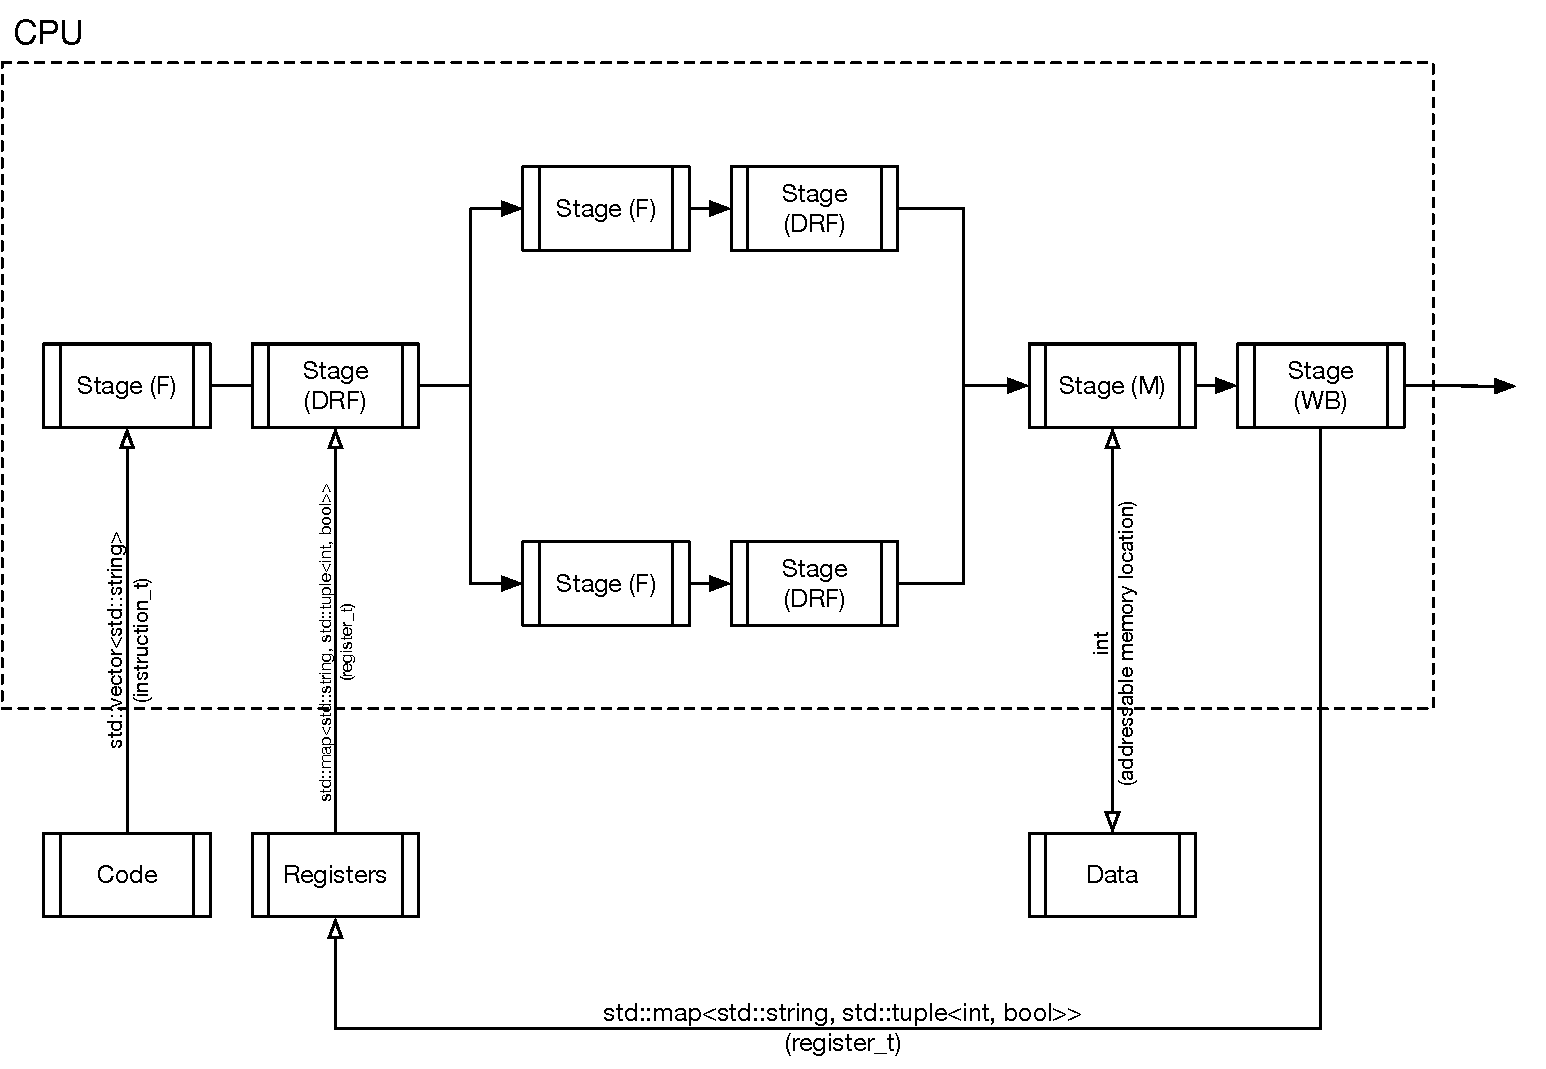
\includegraphics[width=\linewidth]{./figs/apex-sim-overview.pdf}
  \caption{APEX pipeline and class data flows.}
  \label{fig:overview}
\end{figure}

\subsection{Driver Program}
\label{sec:driver}
The \codename entry point file is \texttt{main.cpp}. Besides maintaining simulator state variables for the current cycle, program counter and instructions filename, this program shepherds execution through the lifecycle of the program and provides a user interface for interacting with the simulator. The functionality of the driver program is as follows:
\begin{enumerate}
  \item Verify sanity of command line inputs (lines 107-116).
  \item Instantiate class instances for the simulator (lines 119-122).
  \item Perform the initialization of each pipeline stage (line 125).
  \item Prepare and begin the simulator user interface's operations (lines 128-134).
  \item Parse user interface inputs and delegate actions to interface helper functions (lines 134-161).
\end{enumerate}

\texttt{main.cpp} also provides helper functions which delegate work down to class instances. These functions are:
\begin{itemize}
  \item \texttt{help()} displays the user interface keyboard shortcuts. It's invoked at startup, on request from the user, and whenever the user provides an input which is not recognized.
  \item \texttt{initialize()} resets the simulator state, and invokes the class instances' own \texttt{\textit{classname}.initialize()} functions which reset the instances' internal state.
  \item \texttt{display()} displays the simulator internal state variables as well as delegated calls to each class' \texttt{\textit{classname}.display()} function.
  \item \texttt{quit()} gracefully halts the simulator and triggers a final call to \texttt{display()}.
  \item \texttt{simulate()} is the most important of the helper functions. It is responsible for controlling simulation of the \texttt{CPU.simulate()} function for a given number of cycles, and allowing the CPU class to communicate that it has encountered an error, reached EOF of a code file without a HALT instruction, or has processed a HALT instruction through the pipeline.
\end{itemize}

\subsection{Classes}
\label{sec:classes}
\codename models each major component of the APEX system as a standalone class. These classes are discussed in the following sections.

\subsubsection{Code}
The code class performs two roles.
First, during its construction, it reads a text file into a vector container. This decision was made because random access into a vector is trivial, while random access into a text file whose lines are not a constant length (as in the APEX ISA) is extremely challenging.
Second, those instructions are tokenized by first separating the opcode from its operands by searching for a whitespace character from the beginning of the string, then separating the remainder of the string on commas.

The final result is that the Code class allows us to receive a pre-parsed instruction simply by specifying a program counter value corresponding to a line in the input text file.
As stated in the specification, with a 0-based index, the $k^{th}$ line is the instruction corresponding to program counter value $4000 + 4k$.
Instructions can be easily read into the Fetch stage using the \texttt{std::vector<std::string> Code::getInstr(int addr)} member function.

Unlike the other classes, Code does not provide a means of modifying the values it contains. This is because a code segment is ordinarily not writeable by programs once execution has begun (with exceptions such as Just-In-Time code). \codename models this behavior by prohibiting modifying a Code object after construction. Its contents can be found by reading the source code input text file; accordingly, \codename Code objects do not have a \texttt{display()} method, unlike many of the other component classes.

\subsubsection{Data}
The Data class is similar to the code because it provides the ability for the APEX pipeline to interact with main memory for long-term storage.
(Note: the APEX pipeline does not have a concept of cache levels; the pipeline writes and reads directly from memory).
As a result, Data instances provide an API consisting of two functions: \texttt{int Data::readMem(int addr)} and \texttt{void Data::writeMem(int addr, int value)}.
These function as basic class accessor and mutator respectively.
Because APEX has no concept of memory-to-memory operations, only two Data manipulation instructions exist: LOAD and STORE.
\codename only uses the Data accessor and mutator functions in the Memory (MEM) stage.

Underneath this exposed interface, the Data class uses a vector container consisting of 4000 integer values.
Although 4000 integers exist, in the APEX specification, only 4-byte aligned values are addressable.
Therefore, the unaligned addresses remain unused, and the aligned values of the vector are limited in size to 4 bytes wide (half the width of a 64-bit system integer primitive). This was done for developer convenience, and it is transparent to the user in practice.

\subsubsection{Registers}
\codename models a register file containing infinite virtual read and write ports using the Registers class.
Each register in the register file has three components: a key \-- a string containing the name of the register, and a two-tuple value \-- an integer containing the \textit{value} of the register and a bool containing the \textit{validity}.
The validity of the register is used for simple interlocking as a means of managing flow dependencies across a register.
This (and the process of stalling) is further discussed in section \ref{sec:stalls}.

A Registers instance contains sixteen general purpose registers labelled with the strings "R0" through "R15".
There are also two special purpose registers "X" and "Z".
Strictly speaking, we do not perform any checking for source code which attempts to use these registers.
However, from the Specification, the "X" register is understood to be used to store the most recent return address (i.e. PC + 4) for BAL calls, and the "Z" register is set only as the last arithmetic value calculated in the second ALU (ALU2) stage (i.e. for BZ/BNZ instructions).
These special purpose registers are not to be employed by an APEX programmer for general use.
Forwarding destination set general purpose registers and the "X" and "Z" registers is discussed in section \ref{sec:forwarding}.

The Registers class provides two accessors and one mutator. There are two accessors, one for each of value and validity of a given register key.
The reason for only having one mutator is to require an update of validity each time a value is set in the Write Back (WB) phase.
Underneath this exposed interface, the Registers class is an associative map mapping a string to a two-tuple of integer and bool primitives.
This design decision allows strings representing register names in the assembly code to randomly access values without further translating the string each time to extract the register number, and allows registers to be named without any indication of ordering (i.e. "X" or "Z").
This would have been substantially more difficult with a vector accessed by offset index.

\subsubsection{CPU and Stages}
The CPU class in \codename contains a total of eight instances Stage classes, as described in the Specification. The CPU class therefore serves two purposes.
First, it provides a \texttt{simulate()} function which causes work to occur in each stage.
Second \texttt{simulate()} allows communication between classes for advancing the in-flight instructions and for forwarding.
CPU's delegation and inter-class communication is similar to a Visitor design pattern without abstract class implementations.
This design decision was made solely for expediency.
We acknowledge that a more robust design would use a combination of a Visitor design pattern with threaded instances of each class to simulate simultaneous execution of each stage's work (as opposed to our reverse-order shepherding model, described in section \ref{sec:implementation}).

The \codename CPU class also provides delegation functions which call \texttt{initialize()}, \texttt{display()} on its Stage instances on behalf of \texttt{main.cpp} during simulator execution.

%-----------------------
\section{Implementation}
\label{sec:implementation}
In this section, we will discuss three key aspects of our simulator's execution: the stage-wise reverse-ordered execution, simple interlocking and stalls, and register value forwarding.

\subsection{Stage-wise Reverse Order Execution}
\codename uses stage-wise reverse order execution as a means of simulating the flow of inflight instructions through the pipeline.
This execution consists of two phases using the \texttt{CPU::simulate(...)} function: a working phase (\texttt{simulate.cpp: 9-1138}) and an advancing phase (\texttt{simulate.cpp: 1139-1332}).
What is meant by \textit{stage-wise} is that work is done piecemeal for each phase, and what is meant by \textit{reverse order} is that \codename performs the actions for the WB stage first, then perform actions for each stage in reverse order of the pipeline, with the Fetch (F) stage last.
This has a few benefits.
First, it ensures that an inflight instruction doesn't progress all the way through the pipeline in one advancing phase!
Second, it allows us to model forwarding as the product of a finished stage in the working phase sending its destination register value to an instruction "earlier" in the pipeline.
Third, it ensures that as forwarding occurs, if multiple stages attempt to forward to the same earlier stage, only the most recently computed value remains (earlier values are overwritten).

During the working phase, the \texttt{simulate()} function "visits" each of the stages and performs work specific to the opcode of the inflight instruction "residing" in that stage.
After the work is completed for each stage, it is advanced.
We discuss the process of deciding whether a stage can do work or not in section \ref{sec:stalls}.
In reality, there is no instruction type being sent from stage to stage as a tangible token of inter-stage communication.
Rather, during the advancement phase the contents of one stage are overwritten into the following stage, then the previous stage is marked as \textit{empty} (its contents are not actually deleted as this is an expensive process when it must be done eight times per cycle, and because it is a risk for memory leaks or segmentation faults).
This process occurs using the \texttt{Stage::advance(Stage\& dest)} member function (\texttt{stage.cpp:51-85}).
Additionally, we make a special case for the fetch stage: after a HALT instruction has been received, the Fetch stage continues to fetch NOP instructions to keep the pipeline primed.
Once the HALT instruction is advanced to the WB stage, all stages are marked as empty and execution of the simulator is terminated during the following working phase.

\subsection{Stalls}
\label{sec:stalls}
It is necessary to model instructions stalling in the pipeline.
\codename does this using three mechanisms.
The trivial mechanism is that empty stages don't advance.
This is determined using the Stage's \texttt{isEmpty} field, which is set to false each time a stage advances, and is set to true each time a stage receives an instruction advanced by its predecessor stage (or in the special case of the F stage, each time it fetches the instruction at the program counter's current value).
An instruction cannot advance until its work is completed in a working phase for the stage in which it currently resides.
This knowledge is contained in the Stage class' \texttt{isReady} field, and until a stage is marked as \textit{ready}, it will remain in that stage, stalled.

Also, an instruction cannot do its work until each operand needed for that stage is read and marked \textit{valid} (i.e. no earlier in-flight instructions will update that register's value after a later instruction has read an earlier value from the register file in the DRF stage).
This models the effect of flow dependencies and the solution of simple interlocking, and is done as follows:
Registers in the Register File are marked as invalid as soon as an instruction with that register as a destination exits the DRF stage.
The validity of that destination register is reset when the instruction writes the value to the Register File in the WB stage.
A following instruction's value can be marked valid in one of two ways: it is read from the Register File and the register in the Register File has been reset valid, or it can receive a register value marked \texttt{locally valid} through forwarding.
This \textit{local validity} occurs when the destination register has been computed - for example, the MOVC instruction's destination register becomes \textit{locally valid} upon being computed in the ALU2 stage, but the Register File's instance of that register becomes reset as valid in the later WB stage.

\subsection{Forwarding}
\label{sec:forwarding}
\codename uses data forwarding as a means of reducing delays caused by flow dependencies.
The forwarding paths used by \codename are shown in figure \ref{fig:forwarding}, and a description of each follows. In these descriptions, we consider \textit{arithmetic instructions} to be the set of ADD, SUB, MUL, AND, OR, and EX-OR. We consider the following instructions to have the \textit{source sets} and \textit{destination sets} in table \ref{tab:instsets}.

\begin{table}
  \centering
  \caption{APEX Instruction Source and Destination Sets}
  \label{tab:instsets}
  \begin{tabular}{l|c|c}
    Instruction & Destination Set Operand Indices & Source Set Operand Indices\\
    \hline
    Arithmetic					 	& 0 & 1,2\\
    MOVC 							& 0 & - \\
    LOAD							& 0 & 1 \\
    STORE							& 1 & 0 \\
    BAL, JUMP						& - & 0 \\
    BZ, BNZ 						& - & - \\
    HALT, NOP						& - & - \\
  \end{tabular}
\end{table}

\paragraph{LOAD instruction after Memory stage}
For a LOAD instruction that is exiting the M stage, \codename forwards the contents of its destination register to any arithmetic, MOVC, LOAD, STORE, BAL and JUMP instruction in the DRF, ALU1, ALU2 or B stages that has the same register tag in its sources set. This saves at least one cycle waiting for the instruction to reach and commit its value in the WB stage with the receiving instruction stalled. For a STORE instruction, this permits the STORE instruction to continue in the pipeline, stalling no earlier than when it enters the MEM stage (as opposed to stalling in the DRF stage for its source value).

\paragraph{Arithmetic or MOVC instructions after ALU2 stage}
For an arithmetic instruction exiting the ALU2 stage, \codename forwards the contents of its destination register to any instruction in the ALU1, B, or DRF stages that has the same register tag in its sources set. This saves at least 2 cycles waiting for the instruction to commit its value in the WB stage with the receiving instruction stalled. Furthermore, we speculatively commit the value of the Z register from this stage. This is possible because all instructions which will eventually cause a write to the Z register do so by computing a value, and they do so only in the ALU2 stage and only in program order. Instructions that use the Z value do so in the B stage only, and since they are in that stage, having reached it only after the most recent instruction has calculated Z, we can safely use a speculative commit to simulate forwarding the Z register.

\paragraph{BAL instructions after Branch Stage}
Whenever we take a BAL instruction, we immediately commit the X register's value instead of waiting for the instruction to reach the WB stage. This simulates forwarding the value of the X register from the B stage to the register file. This is possible because only one stage (B) writes to that register, and only one instruction (BAL) is capable of triggering such a write.

\begin{figure}
  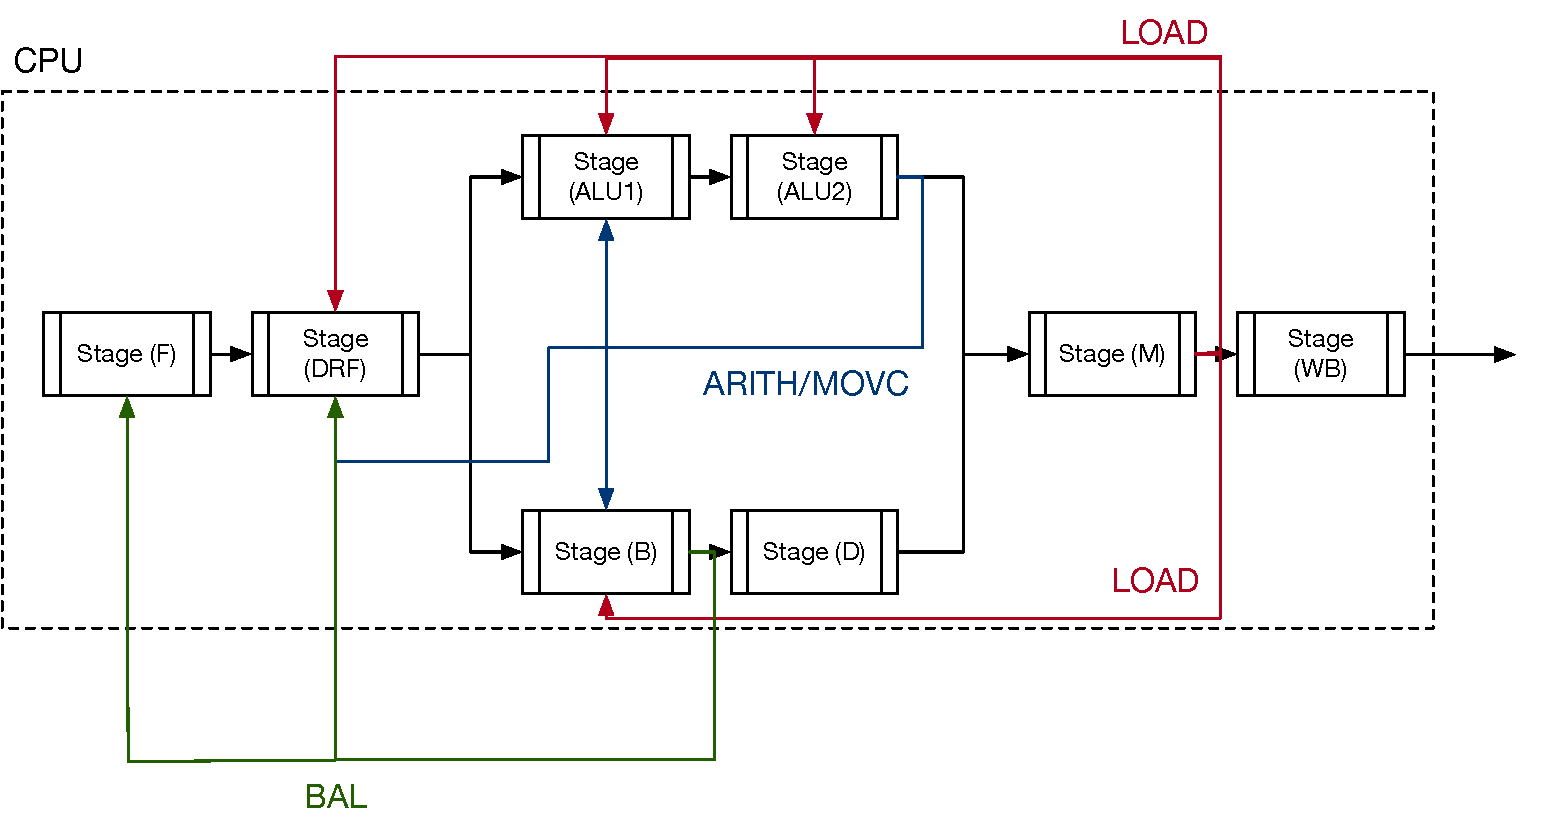
\includegraphics[width=\linewidth]{./figs/apex-sim-forwarding.pdf}
  \caption{APEX pipeline forwarding paths.}
  \label{fig:forwarding}
\end{figure}

%-------------------
\section{Work Log}
\label{sec:worklog}
We open-sourced \codename under the MIT license, and developed it using a GitHub repository. \footnote{The repository is available at \url{https://github.com/colematt/apex-sim}}
This repository contains this documentation, all source code, reference materials on the APEX ISA semantics, and other related materials.
Additionally, it contains an in-depth look at our work progress over the course of this project at a much finer grain than this report contains.
As of writing this report, 90 commits were made, for a total of just under 7500 lines of code added.
Naturally, such a volume of code and the required levels of collaboration would have been nearly impossible without the use of some sort of repository.
We encourage the curious reader to see these statistics in depth using the \textbf{Pulse} and \textbf{Graphs} tabs available on the repository.

Table \ref{tab:worklog} is a broad, chronological overview of work performed by each member.

\begin{table}
\centering
\caption{Chronological Work Log}
\label{tab:worklog}
\begin{tabular}{l|p{2.75in}|p{2.75in}}
Date         	& Matthew's Task
							& Brian's Task \\
\hline
Oct 26, 2016 	& Initial repository setup
							& \\
Oct 29, 2016 	& Initial file push, wrote Makefile
							& \\
Oct 30, 2016 	& Driver program structured
							& \\
Oct 31, 2016 	& Driver program user interface
							&  \\
Nov 8, 2016  	&
							& Code and Data classes structured \\
Nov 10, 2016 	& Initial work on Register File
							& \\
Nov 12, 2016 	& Class Display functions, exception handling, register file
							& Header files corrected; guards added, initial build and troubleshooting \\
Nov 13, 2016 	& Documentation and report; CPU class boilerplate
							& Instruction parsing corrections, CPU class operations \\
Nov 14, 2016 	& CPU Pipelining
							& Compilation tests, updated Code class to reflect new byte addressability standard \\
Nov 15, 2016 	& Reverse-order pipeline, inter-class communications within pipeline; wrote source set,destination set tag membership tests
							& Continued work on pipeline operations \\
Nov 16, 2016 	& Squashed bugs in pipeline
							& Continued work on pipeline operations \\
Nov 17, 2016 	& Added quitting functionality, wrote test cases, added advance function to reduce code redundancy
							& Updated logic for setting register validity (squashed bugs!) Corrected pointer/non-pointer errors in references, improved Work phase for execution efficiency \\
Nov 18, 2016 	& Finished documentation.
							& Completed pipelining. Completed forwarding. Screen captures of working product. \textbf{Checkpointed Release 1.0!} \\
Nov 19, 2016 	& Final repository pushes. \textbf{Checkpointed Release 1.1!}
							& \\
Dec 4, 2016  	& \textbf{Checkpointed Release 1.2!}
							&  \\
\end{tabular}
\end{table}


%---------------
\newpage
\appendix
\section{Appendix: Screen Captures}
\begin{figure}
  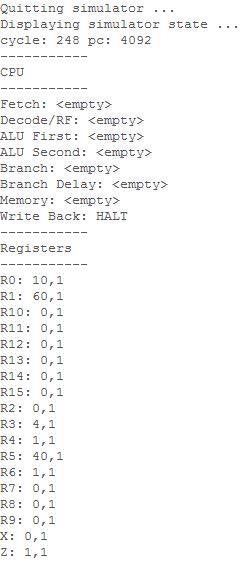
\includegraphics{./figs/sti1pipereg.jpg}
  \caption{Final Pipeline Contents and Register File of SimpleTestInput1}
  \label{fig:sti1pipereg}
\end{figure}
\begin{figure}
  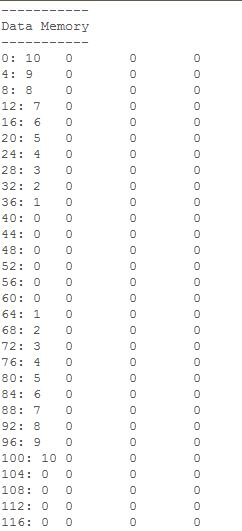
\includegraphics{./figs/sti1mem.jpg}
  \caption{Final Memory Contents of SimpleTestInput1}
  \label{fig:sti1mem}
\end{figure}
\begin{figure}
  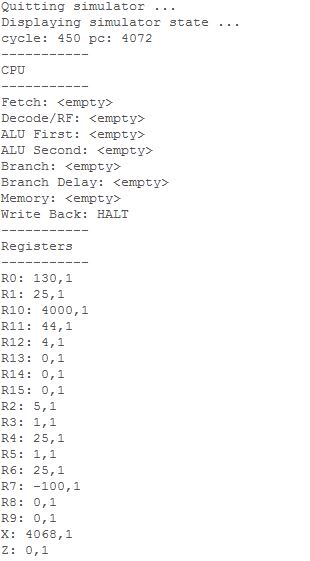
\includegraphics{./figs/sti2pipereg.jpg}
  \caption{Final Pipeline Contents and Register File of SimpleTestInput2}
  \label{fig:sti2pipereg}
\end{figure}
\begin{figure}
  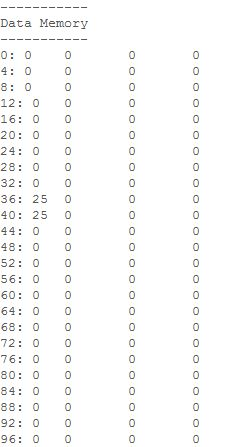
\includegraphics{./figs/sti2mem.jpg}
  \caption{Final Memory Contents of SimpleTestInput2}
  \label{fig:sti2mem}
\end{figure}

\end{document}
